% !TeX spellcheck = ru_RU
% !TeX encoding = UTF-8
\section{Технология «СТРИЖ»}
\subsubsection{Назначение}
«СТРИЖ» — это беспроводная система сбора, передачи и обработки данных счетчиков, датчиков и приборов учета для ЖКХ, электроэнергетики и систем безопасности.

«СТРИЖ Телематика» разрабатывает и продвигает новый класс устройств, работающих по стандарту LPWAN (Low-Power Wide-Area Network). Эти устройства могут автономно работать на одной батарейке многие годы, передавая сигнал по радиоканалу на большие расстояния. 


К настоящему времени компания разработала и начала внедрение несколько типов устройств, которые используются для передачи данных в различных областях. В секторе ЖКХ — это счетчики воды и электричества, передающие показания, а также модемы для передачи показаний счетчиков воды, газа, электричества и тепла. Для сферы сельского хозяйства выпущены датчики влажности почвы для открытых полей большой площади и закрытых теплиц, термоштанга для контроля сохранности урожая через мониторинг температуры и датчик углекислого газа для контроля сохранности урожая через мониторинг концентрации диоксида углерода. В процессе разработки находится серия интегрированных устройств для учета тепла и охраны банкоматов.

\subsubsection{Структура системы}
Рассмотрим структуру системы «СТРИЖ». Типичная сеть «СТРИЖ» состоит из следующих элементов: 
\begin{itemize}
	\item"Датчики". Специальные устройства для сбора данных, изготовленные компанией «СТРИЖ Телематика».  
	\item"Приёмники". В технологии «СТРИЖ» используется термин "Базовая станция".
	\item"Пункт сбора". В технологии «СТРИЖ» используется термин "сервер «СТРИЖ»".
	\item Облачный сервер. С сервера «СТРИЖ» данные передаются либо в личный кабинет пользователя "в облаке", либо на сервер клиента.
\end{itemize}
Структурная схема системы представлена на рисунке
\ref{fig:Swift}.

\begin{figure}[H]
	\centering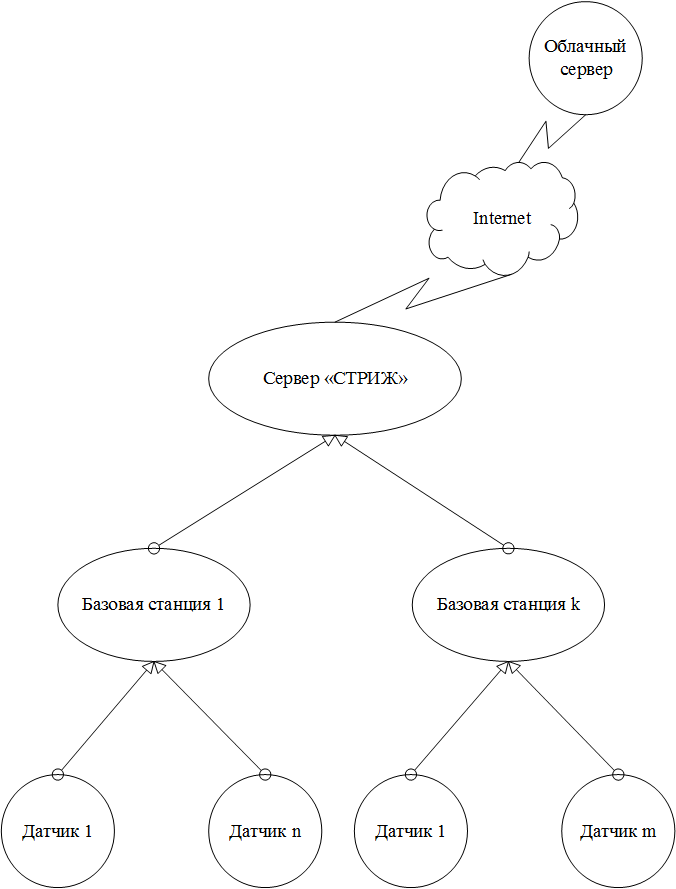
\includegraphics[width=0.7\linewidth]{img/Swift}
	\caption{Структурная схема системы, построенной по технологии «СТРИЖ»}
	\label{fig:Swift}
\end{figure}

Подход, используемый для передачи данных в сети «СТРИЖ», очень похож на принцип работы сотовых сетей.

Устройства «СТРИЖ» передают показания в личный кабинет клиента через базовую станцию, где они обрабатываются и предоставляются в удобном для пользователя виде. Обратный канал позволяет управлять отдельными приборами удаленно\cite{2}.

Однако, в отличие от технологии мобильной связи, «СТРИЖ» использует свой энергоэффективный радиопротокол, что позволяет передавать данные на расстояния до 50 км и обеспечить автономность работы устройств свыше 10 лет без внешнего питания.


\subsubsection{Разбиение системы на уровни}

Способ разбиения системы «СТРИЖ» на уровни представлен на рисунке
\ref{fig:system_levels_1}.
\begin{figure}[H]
	\centering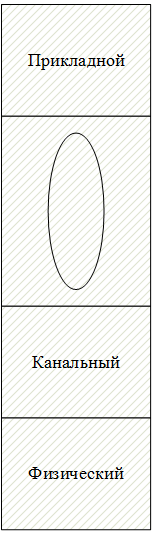
\includegraphics[width=0.2\linewidth]{img/system_levels_1}
	\caption{Разбиение на уровни системы «СТРИЖ»}
	\label{fig:system_levels_1}
\end{figure}

\subsubsection{Особенности построения уровней}
Главной особенностью построения уровней системы «СТРИЖ» является то, что все уровни данной системы являются закрытыми.
 
Особенностью физического уровня системы можно считать то, что устройства и модемы «СТРИЖ» не требуют подключения к электросети. Они вообще не требовательны к питанию. Процесс отправки данных оптимизирован, а мощность передачи в 80 раз ниже, чем у мобильного телефона. Именно поэтому одного источника питания хватает на 10 лет работы прибора.